%**************************************************************************************
% License:
% CC BY-NC-SA 4.0 (http://creativecommons.org/licenses/by-nc-sa/4.0/)
%**************************************************************************************

\documentclass[notes]{beamer}

\mode<presentation> {

\usetheme{Madrid}

% Burnt orange
\definecolor{burntorange}{rgb}{0.8, 0.33, 0.0}
\colorlet{beamer@blendedblue}{burntorange}
% Pale yellow
\definecolor{paleyellow}{rgb}{1.0, 1.0, 0.953}
\setbeamercolor{background canvas}{bg=paleyellow}
% Secondary and tertiary palett
\setbeamercolor*{palette secondary}{use=structure,fg=white,bg=burntorange!80!black}
\setbeamercolor*{palette tertiary}{use=structure,fg=white,bg=burntorange!60!black}

% To remove the footer line in all slides uncomment this line
%\setbeamertemplate{footline}
% To replace the footer line in all slides with a simple slide count uncomment this line
%\setbeamertemplate{footline}[page number]

% To remove the navigation symbols from the bottom of all slides uncomment this line
%\setbeamertemplate{navigation symbols}{}
}

\usepackage{amsmath}
\usepackage{bm}
\usepackage{breqn}
\usepackage{graphicx} % for figures
\usepackage{subcaption} % for subplots 
\usepackage[labelsep=space,tableposition=top]{caption}
\renewcommand{\figurename}{Fig.} 
\usepackage{cleveref}
\usepackage{caption,subcaption}% http://ctan.org/pkg/{caption,subcaption}
\usepackage{booktabs} % Allows the use of \toprule, \midrule and \bottomrule in tables
\usepackage{multirow}

% To print 2 slides on a page
%\usepackage{handoutWithNotes}
%\pgfpagesuselayout{2 on 1}[border shrink=2mm]
%----------------------------------------------------------------------------------------
%	TITLE PAGE
%----------------------------------------------------------------------------------------
% The short title appears at the bottom of every slide, the full title is only on the title page
\title[CE394M: isoparametric - gauss integration]{CE394M: Isoparametric elements and Gauss integration} 
\author{Krishna Kumar} % name
\institute[UT Austin] % institution 
{
University of Texas at Austin \\
\medskip
\textit{
  \url{krishnak@utexas.edu}} % Your email address
}
\date{\today} % Date, can be changed to a custom date

\begin{document}

\begin{frame}
\titlepage % title page as the first slide
\end{frame}

\begin{frame}
 % Table of contents slide, comment this block out to remove it
 \frametitle{Overview}
 % Throughout your presentation, if you choose to use \section{} and \subsection{} 
 % commands, these %will automatically be printed on this slide as an overview 
 \tableofcontents
\end{frame}

%----------------------------------------------------------------------------------------
% slides
%----------------------------------------------------------------------------------------
\section{Rectangular elements}
%------------------------------------------------
\begin{frame}
\frametitle{4-noded rectangular element}
An alternative and more elegant approach is to construct the shape functions by the \textbf{tensor
product method.} This is based on taking products of one-dimensional shape functions.

\begin{figure}[ht]
	\centering
	\includegraphics[width=0.8\textwidth]{figs/4noded-quad-tensor-product.png}
	\caption*{Construction of two dimensional shape functions.}
\end{figure}
\begin{equation*}
N_2^e = N_2^{e,1d}(x) \times N_1^{e,1d}(y)
\end{equation*}

\end{frame}

%------------------------------------------------
\begin{frame}
\frametitle{4-noded rectangular element}

The four shape functions, also called \textbf{bilinear shape functions}, for the quadrilateral element are:
\begin{align*}
	N_1^e (x, y) & = \frac{x - x_2^e}{x_1^e - x_2^e}\frac{y - y_4^e}{y_1^e - y_4^e} = \frac{1}{A^e}(x - x_2^e)(y - y_4^e) \\
	%
	N_2^e (x, y) & = \frac{x - x_1^e}{x_2^e - x_1^e}\frac{y - y_4^e}{y_1^e - y_4^e} = -\frac{1}{A^e}(x - x_1^e)(y - y_4^e) \\
	%
	N_3^e (x, y) & = \frac{x - x_1^e}{x_2^e - x_1^e}\frac{y - y_1^e}{y_4^e - y_1^e} = \frac{1}{A^e}(x - x_1^e)(y - y_1^e) \\
	%
	N_4^e (x, y) & = \frac{x - x_2^e}{x_1^e - x_2^e}\frac{y - y_1^e}{y_4^e - y_1^e} = -\frac{1}{A^e}(x - x_2^e)(y - y_1^e)\\
\end{align*}

where $A^e$ is the area of the element.

\end{frame}


%------------------------------------------------
\begin{frame}
\frametitle{4-noded rectangular element}
The four shape functions are plotted in the following
figure:
\begin{figure}[ht]
	\centering
	\includegraphics[width=\textwidth]{figs/4noded-sf.png}
	\caption*{Four shape functions of the rectangular element (on $[0, 2] \times [0, 2]$).}
\end{figure}
\end{frame}


%------------------------------------------------
\begin{frame}
\frametitle{4-noded rectangular element}
If the sf equations are used for interpolating the temperature field over arbitrary quadrilaterals, the scalar field (e.g., temperature) across the element boundaries will be not continuous.
\begin{figure}[ht]
	\centering
	\includegraphics[width=\textwidth]{figs/discontinous-rectangle.png}
	\caption*{Two element mesh with rectangle shape functions. Although the two nodal values on the
		edge agree, the temperature distribution is still discontinuous.}
\end{figure}
\end{frame}

\note{
	The computed shape functions are suitable for rectangles and could be used with meshes consisting only of rectangles, but they are not suitable for arbitrary quadrilaterals.
	
	Therefore, these shape functions are of limited use for practical applications. To obtain
	the shape functions for arbitrary quadrilaterals we need to visit the idea of isoparametric
	mapping.
}

%------------------------------------------------
\section{Isoparametric elements}
%------------------------------------------------
\begin{frame}
\frametitle{Isoparametric mapping in 1D}
\mode<beamer>{
	\begin{figure}[ht]
		\centering
		\includegraphics[width=0.85\textwidth]{figs/1d-isoparametric.png}
	\end{figure}
}
\mode<handout>{
	\vspace{5cm}
}
\end{frame}
\note{Although isoparametric mapping is not particularly useful in one dimension, it is very	helpful for understanding the general approach.
}

%------------------------------------------------
\begin{frame}
\frametitle{Isoparametric mapping in 1D}
consider a coordinate transformation which transforms (maps) the coordinate $x$ into a local (element specific) coordinate $\xi$:	
\begin{figure}[ht]
	\centering
	\includegraphics[width=0.85\textwidth]{figs/1d-isoparametric-shapefn.png}
\end{figure}
The coordinate $\xi$ fulfills the relationships:

\mode<beamer>{
	$x = x^e_1$ at $\xi = -1$ and $x = x^e_2$ at $\xi=1$
}
\mode<handout>{
	\vspace{1cm}
}

``stretch transformation'' of $x(\xi)$: 

\mode<beamer>{
	\begin{align*}
		x(\xi) & = x_1^e + \frac{1}{2}(x_2^e - x_1^e)(1+\xi) \\
			& = \frac{x_1^e + x_2^e}{2} + \frac{x_2^e - x_1^e}{2}\xi
	\end{align*}
}
\mode<handout>{
	\vspace{1cm}
}
\end{frame}


%------------------------------------------------
\begin{frame}
\frametitle{Isoparametric mapping in 1D}
The shape functions $N_1^e = (1 - x/l)$ and $N_2^e = (x/l)$ can also be expressed using $\xi$:
\mode<beamer>{
	\begin{equation*}
		N_1^e(\xi) = \frac{1}{2}(1-\xi) \qquad N_2^e(\xi) = \frac{1}{2}(1+\xi)
	\end{equation*}
}
\mode<handout>{
	\vspace{1cm}
}

The key idea of the isoparametric concept is to use these shape functions for writing the
coordinate transformation between $x$ and $\xi$ 

\mode<beamer>{
	\begin{align*}
	x(\xi) & = N_1^e(\xi)x_1^e + N_2^e(\xi)x_2^e  \\
		   & = \frac{1}{2}(1-\xi) x_1^e + %
		    \frac{1}{2}(1+\xi) x_2^e \\
		   & = \frac{x_1^e + x_2^e}{2} + \frac{x_2^e - x_1^e}{2}\xi
	\end{align*}
}
\mode<handout>{
	\vspace{3cm}
}
\begin{figure}[ht]
	\centering
	\includegraphics[width=0.65\textwidth]{figs/1d-isoparametric-shapefn.png}
\end{figure}
\end{frame}


%------------------------------------------------
\begin{frame}
\frametitle{Isoparametric mapping in 1D}

\begin{itemize}
	\item The coordinate $\xi$ is usually called the \textbf{natural coordinate} and always lies by definition between -1 and +1.
	
	\item The parent element is solely for numerical purposes. 
	
	\item The finite element analysis is still performed over the physical domain.
\end{itemize}


In an isoparametric element the field variable, like displacement, is approximated with the
same set of shape functions as those used for the coordinate transformation:

\mode<beamer>{
	\begin{equation*}
	u(\xi) = N_1^e(\xi)a_1^e + N_2^e(\xi)a_2^e  
	\end{equation*}
}
\mode<handout>{
	\vspace{1cm}
}

To compute the derivatives which appear in the weak form the chain rule is used:

\mode<beamer>{
	\begin{equation*}
		\frac{du}{dx} = \frac{du}{d\xi}\frac{d\xi}{dx}
	\end{equation*}
	The derivative $d\xi/dx$ is determined from the mapping between $\xi$ and $x$
}
\mode<handout>{
	\vspace{1cm}
}
\end{frame}


%------------------------------------------------
\section{Isoparametric quadrilateral elements}
%------------------------------------------------
\begin{frame}
\frametitle{Isoparametric mapping of a quadrilateral element}
The idea of isoparametric mapping is used for deriving shape functions for arbitrary quadrilateral elements:
\begin{figure}[ht]
	\centering
	\includegraphics[width=\textwidth]{figs/2d-isoparametric-shapefn.png}
\end{figure}
\end{frame}

%------------------------------------------------
\begin{frame}
\frametitle{Isoparametric mapping of a quadrilateral element}
The bi-unit square is the parent domain and $\xi$ and $\eta$ are its natural coordinates. 

To map points from the parent domain onto the quadrilateral in the physical domain the four nodal
shape functions are used:

\mode<beamer>{
	\begin{equation*}
	x(\xi, \eta) = \mathbf{N}^{4Q}(\xi, \eta)x^e \quad
	y(\xi, \eta) = \mathbf{N}^{4Q}(\xi, \eta)y^e
	\end{equation*}
	where $N^{4Q}(\xi, \eta)$ are the four-node element shape functions in the natural coordinates and $x^e$ and $y^e$ are the vectors of the element coordinates:
	\begin{equation*}
	\mathbf{x}^e = 
	\begin{bmatrix} 
	x_1^e \\
	x_2^e \\
	x_3^e \\
	x_4^e \\
	\end{bmatrix}
	\quad
	\mathbf{y}^e = 
	\begin{bmatrix} 
	y_1^e \\
	y_2^e \\
	y_3^e \\
	y_4^e \\
	\end{bmatrix}
	\end{equation*}
	
}
\mode<handout>{
	\vspace{5cm}
}
\end{frame}

%------------------------------------------------
\begin{frame}
\frametitle{Isoparametric mapping of a quadrilateral element}
As the parent element is a bi-unit square its shape functions are identical to those of the
rectangular element expressed in $\xi$ and $\eta$ coordinates.
\begin{align*}
	N_1^{4Q}(\xi, \eta) & = \frac{1}{4}(1-\xi)(1-\eta)\\
	N_2^{4Q}(\xi, \eta) & = \frac{1}{4}(1+\xi)(1-\eta)\\
	N_3^{4Q}(\xi, \eta) & = \frac{1}{4}(1+\xi)(1+\eta)\\
	N_4^{4Q}(\xi, \eta) & = \frac{1}{4}(1-\xi)(1+\eta)\\
\end{align*}
\end{frame}


%------------------------------------------------
\begin{frame}
\frametitle{Isoparametric shape functions}
The temperature will be approximated with the same shape functions:

\mode<beamer>{
	\begin{equation*}
		T^e = \mathbf{N}^{4Q}(\xi, \eta) \mathbf{a}^e
	\end{equation*}
}
\mode<handout>{
	\vspace{1cm}
}
The element is called \textit{isoparametric} because the temperature approximation and the mapping of the geometry is accomplished with the same shape functions.

The displacement will be approximated as:
\mode<beamer>{
	\begin{align*}
	\mathbf{u}^e & = \mathbf{N}^{4Q}(\xi, \eta) \mathbf{a}^e \\
	& = \begin{bmatrix}
	N_1^{4Q} & 0 & N_2^{4Q} & 0 & N_3^{4Q} & 0 & N_4^{4Q} & 0 \\
	0 & N_1^{4Q} & 0 & N_2^{4Q} & 0 & N_3^{4Q} & 0 & N_4^{4Q} \\
	\end{bmatrix}
	\begin{bmatrix}
		a_{1x}^e \\
		a_{1y}^e \\
		a_{2x}^e \\
		a_{2y}^e \\
		a_{3x}^e \\
		a_{3y}^e \\
		a_{4x}^e \\
		a_{4y}^e \\
	\end{bmatrix}
	\end{align*}
}
\mode<handout>{
	\vspace{3cm}
}
\end{frame}

%------------------------------------------------
\begin{frame}
\frametitle{Derivatives isoparametric shape functions}
The gradient of displacement for the four-node (isoparametric) quadrilateral element is:

	Strain:	$\epsilon = \mathbf{B}^{e}\mathbf{a}^e$
	
	\begin{equation*}
	\begin{bmatrix}
		\epsilon_{xx}^e \\
		\epsilon_{yy}^e \\
		2\epsilon_{xy}^e \\
	\end{bmatrix}	 = %
	\begin{bmatrix}
		\frac{\partial N_1^{4Q}}{\partial x} & 0 &
		\frac{\partial N_2^{4Q}}{\partial x} & 0 &
		\frac{\partial N_3^{4Q}}{\partial x} & 0 &
		\frac{\partial N_4^{4Q}}{\partial x} & 0 \\
		0 &	\frac{\partial N_1^{4Q}}{\partial y} & 
		0 &	\frac{\partial N_2^{4Q}}{\partial y} &
		0 &\frac{\partial N_3^{4Q}}{\partial y} &
		0 & \frac{\partial N_4^{4Q}}{\partial y} \\	
		\frac{\partial N_1^{4Q}}{\partial y} & \frac{\partial N_1^{4Q}}{\partial x} &  
		\frac{\partial N_2^{4Q}}{\partial y} &
		\frac{\partial N_2^{4Q}}{\partial x} &
		\frac{\partial N_3^{4Q}}{\partial y} &
		\frac{\partial N_3^{4Q}}{\partial x} & 
		\frac{\partial N_4^{4Q}}{\partial y} &
		\frac{\partial N_4^{4Q}}{\partial x} & \\
	\end{bmatrix}
	\begin{bmatrix}
		u_{1x}^e \\
		u_{1y}^e \\
		u_{2x}^e \\
		u_{2y}^e \\
		u_{3x}^e \\
		u_{3y}^e \\
		u_{4x}^e \\
		u_{4y}^e \\
	\end{bmatrix}
	\end{equation*}
\end{frame}

%------------------------------------------------
\begin{frame}
\frametitle{Derivatives isoparametric shape functions}
To compute shape function derivatives the chain rule will be used:

\mode<beamer>{
	\begin{align*}
		\frac{\partial N_I^{4Q}}{\partial \xi} & = \frac{\partial N_I^{4Q}}{\partial x} \frac{\partial x}{\partial \xi} + %
		\frac{\partial N_I^{4Q}}{\partial y} \frac{\partial y}{\partial \xi} \\
	%
		\frac{\partial N_I^{4Q}}{\partial \eta} & = \frac{\partial N_I^{4Q}}{\partial x} \frac{\partial x}{\partial \eta} + %
		\frac{\partial N_I^{4Q}}{\partial y} \frac{\partial y}{\partial \eta} \\
	\end{align*}
}
\mode<handout>{
	\vspace{2cm}
}
written as matrices and vectors this becomes:
\mode<beamer>{
	\begin{equation*}
	\begin{bmatrix}
		\frac{\partial N_I^{4Q}}{\partial \xi} \\
		\frac{\partial N_I^{4Q}}{\partial \eta} \\
	\end{bmatrix}
	=% 
	\begin{bmatrix}
		\frac{\partial x}{\partial \xi} & \frac{\partial y}{\partial \xi} \\
		\frac{\partial x}{\partial \eta} & \frac{\partial y}{\partial \eta} \\
	\end{bmatrix}
	\begin{bmatrix}
		\frac{\partial N_I^{4Q}}{\partial x} \\
		\frac{\partial N_I^{4Q}}{\partial y} \\
	\end{bmatrix}
	\end{equation*}
}
$\mathbf{J}^e$ is the Jacobian which contains the derivatives of the physical coordinates with respect
to the natural coordinates.
\mode<handout>{
	\vspace{3cm}
}
\end{frame}

%------------------------------------------------
\begin{frame}
\frametitle{Derivatives isoparametric shape functions}
The derivatives required for the weak form are computed by
inverting the above expression:
\mode<beamer>{
	\begin{equation*}
	\begin{bmatrix}
		\frac{\partial N_I^{4Q}}{\partial x} \\
		\frac{\partial N_I^{4Q}}{\partial y} \\
	\end{bmatrix}
	= %
	(\mathbf{J}^e)^{-1}
	\begin{bmatrix}
	\frac{\partial N_I^{4Q}}{\partial \xi} \\
	\frac{\partial N_I^{4Q}}{\partial \eta} \\
	\end{bmatrix}
	\end{equation*}
}
\mode<handout>{
	\vspace{2.5cm}
}
The inverse of $\mathbf{J}^e$ is:
\mode<beamer>{
	\begin{equation*}
	{\mathbf{J}^e}^{-1}
	= \frac{1}{\left| \mathbf{J}^e\right|}
	\begin{bmatrix}
		\frac{\partial y}{\partial \eta} & -\frac{\partial y}{\partial \xi} \\
		-\frac{\partial x}{\partial \eta} & \frac{\partial y}{\partial \xi} \\
	\end{bmatrix}
	\end{equation*}
}
\mode<handout>{
	\vspace{2.5cm}
}
Where $\left|\mathbf{J}^e\right|$ is the determinant of the Jacobian, which represents the ratio of an area element in the physical domain to the corresponding area element in the parent domain.
\end{frame}


%------------------------------------------------
\begin{frame}
	\frametitle{Jacobian}
	The Jacobian can also be thought of as describing the amount of ``stretching'', ``rotating'' or ``transforming'' that a transformation imposes locally. For example, if $(x^\prime, y^\prime) = f(x, y)$ is used to transform an image, the Jacobian $\mathbf{J} f(x, y)$, describes how the image in the neighborhood of $(x, y)$ is transformed.
	
	\begin{figure}[ht]
		\centering
		\includegraphics[width=0.6\textwidth]{figs/jacobian.png}
		\caption*{The Jacobian at a point gives the best linear approximation of the distorted parallelogram near that point (in translucent white on the right-side), and the Jacobian determinant gives the ratio of the area of the approximating parallelogram to that of the original square.}
	\end{figure}
\end{frame}

%------------------------------------------------
\begin{frame}
\frametitle{Derivatives isoparametric shape functions}
The isoparametric mapping is used to compute the Jacobian:
\mode<beamer>{
	\begin{equation*}
	x(\xi, \eta) = \mathbf{N}^{4Q}(\xi, \eta)\mathbf{x}^e \quad
	y(\xi, \eta) = \mathbf{N}^{4Q}(\xi, \eta)\mathbf{y}^e \quad
	\end{equation*}
}
\mode<handout>{
	\vspace{3cm}
}
which leads to:
\begin{equation*}
	\mathbf{J}^e = %
	\begin{bmatrix}
		\frac{\partial N_1^{4Q}}{\partial \xi} &
		\frac{\partial N_2^{4Q}}{\partial \xi} &
		\frac{\partial N_3^{4Q}}{\partial \xi} &
		\frac{\partial N_4^{4Q}}{\partial \xi} \\
		\frac{\partial N_1^{4Q}}{\partial \eta} &
		\frac{\partial N_2^{4Q}}{\partial \eta} &
		\frac{\partial N_3^{4Q}}{\partial \eta} &
		\frac{\partial N_4^{4Q}}{\partial \eta} \\	
	\end{bmatrix}
	\begin{bmatrix}
		x_1^e & y_1^e\\
		x_2^e & y_2^e\\
		x_3^e & y_3^e\\
		x_4^e & y_4^e\\
	\end{bmatrix}
\end{equation*}
\end{frame}

%------------------------------------------------
\begin{frame}
\frametitle{Higher order quadrilateral element}

\begin{figure}[ht]
	\centering
	\includegraphics[width=0.85\textwidth]{figs/9noded-quadrilateral.png}
	\caption*{Nine-node ispoarametric quadrilateral in parameter (left) and physical space (right).}
\end{figure}
\end{frame}
\note{
	Higher order quadrilateral elements provide the ability to model curved edges. The advantage of curved edges is that fewer elements can be used around holes and other curved surfaces than with straight-sided elements. \\
	
	The nine-node isoparametric element is constructed as a tensor product of the one-dimensional quadratic shape functions. The $\mathbf{B}_e$ matrix for the nine noded element is computed with the same approach as discussed in the previous section.
}

\section{Effect of element shape}
%------------------------------------------------
\begin{frame}
\frametitle{Effect of element shape on isoparametric mapping}
Consider the following isoparametric mapping for a four-node quadrilateral element:
\begin{figure}[ht]
	\centering
	\includegraphics[width=\textwidth]{figs/2d-isoparametric-example.png}
\end{figure}
\end{frame}

%------------------------------------------------
\begin{frame}
\frametitle{Effect of element shape on isoparametric mapping}
The Jacobian of this mapping:
\begin{equation*}
	\mathbf{J}^e%
	=% 
	\begin{bmatrix}
		\frac{\partial x}{\partial \xi} & \frac{\partial y}{\partial \xi} \\
		\frac{\partial x}{\partial \eta} & \frac{\partial y}{\partial \eta} \\
	\end{bmatrix}
\end{equation*}
is computed from
\mode<beamer>{
	\begin{align*}
		x & = 0.0 N_1^{4Q} + 5.0  N_2^{4Q} + 3.0  N_3^{4Q} + 0.0  N_4^{4Q} \\
		% 
		& = 2 \xi - \frac{1}{2}\eta - \frac{1}{2}\xi \eta + 2 \\
		%
		\vspace{1em}
		%
		y & = 0.0 N_1^{4Q} + 0.0  N_2^{4Q} + 3.0  N_3^{4Q} + 5.0  N_4^{4Q} \\
		% 
		& = - \frac{1}{2} \xi + 2 \eta - \frac{1}{2}\xi \eta + 2 \\
	\end{align*}
}
\mode<handout>{
	\vspace{4cm}
}
\end{frame}


%------------------------------------------------
\begin{frame}
\frametitle{Effect of element shape on isoparametric mapping}
After some algebra we obtain:
\begin{equation*}
\mathbf{J}^e%
=% 
\begin{bmatrix}
2 - \frac{\eta}{2} & -\frac{1}{2} -\frac{1}{2}\eta \\
 -\frac{1}{2} -\frac{1}{2}\xi & 2 - \frac{1}{2}\xi \\
\end{bmatrix}
\end{equation*}

The Jacobian has to be invertible for computing the derivatives of the shape functions with
respect to the physical coordinates.

For the mapping to be invertible, the determinant of the Jacobian has to be larger than zero over the entire element:

\mode<beamer>{
	\begin{equation*}
		det \mathbf{J}^e = \frac{5}{4}(3 - \xi - \eta) > 0
	\end{equation*}
}
\mode<handout>{
	\begin{equation*}
	det \mathbf{J}^e = \frac{5}{4}(3 - \xi - \eta)
	\end{equation*}
}
which is the case for this mapping.
\end{frame}


%------------------------------------------------
\begin{frame}
\frametitle{Effect of element shape on isoparametric mapping}
In contrast to the previous mapping, it can be for the following mapping shown:
\begin{figure}[ht]
	\centering
	\includegraphics[width=\textwidth]{figs/2d-isoparametric-example-negative-jacobian.png}
\end{figure}
that the determinant of the Jacobian is zero or negative close to the non-convex corner.
\end{frame}

\note{
	Notice that some region of the parent element close to node 3 is mapped outside the
	physical domain. If such non-convex elements are present in the finite element mesh, the
	results of the finite element computation will be useless.
}

%------------------------------------------------
\section{Numerical Integration (Quadrature)}
%------------------------------------------------
\begin{frame}
\frametitle{Numerical integration (Quadrature)}
\begin{itemize}
	\item During the finite element solution procedure, it is necessary to integrate various quantities,	for instance the stiffness matrix or force vectors. 
	\item For isoparametric elements these
	quantities must in general be integrated numerically due to the presence of the Jacobian.
	\item Although there are many different numerical integration techniques, in finite elements
	Gauss integration is preferred.
\end{itemize}
\end{frame}

%------------------------------------------------
\begin{frame}
\frametitle{Review of Basic Integration Rules}
Consider the following integral which is to be integrated numerically:

\begin{equation*}
	\int_a^b f(x)dx
\end{equation*}

The integration domain $[a, b]$ is first split into $N$ equidistant subintervals:

\mode<beamer>{
	\begin{equation*}
		x_I = a + I h
	\end{equation*}
}
\mode<handout>{
	\vspace{1.5cm}
}
with:
\mode<beamer>{
	\begin{equation*}
		h = \frac{b - a}{N} \quad I = 0, 1, \dots, N
	\end{equation*}
}
\mode<handout>{
	\vspace{1.5cm}
}
There are various schemes for approximating the integral using the function values at $N$ positions
\end{frame}

%------------------------------------------------
\begin{frame}
\frametitle{Rectangle rule (constant approximation)}
\mode<beamer>{
	\begin{figure}[ht]
		\centering
		\includegraphics[width=\textwidth]{figs/rectangle-rule-integration.png}
	\end{figure}
}
\mode<handout>{
	\vspace{3.5cm}
}
Integration of $f(x)$ with the rectangle rule between $x = a$ and $x = b$.
\mode<beamer>{
	\begin{equation*}
	\int_a^b f(x)dx \approx h (f(x_0) + f(x_1)+f(x_2)+\dots+f(x_{N-1}))
	\end{equation*}
}
\mode<handout>{
	\vspace{1cm}
}
\end{frame}

%------------------------------------------------
\begin{frame}
\frametitle{Trapezoidal rule (linear approximation)}
\mode<beamer>{
	\begin{figure}[ht]
		\centering
		\includegraphics[width=\textwidth]{figs/trapezoidal-rule-integration.png}
	\end{figure}
}
\mode<handout>{
	\vspace{3.5cm}
}
Integration of $f(x)$ with the trapezoidal rule between $x = a$ and $x = b$.
\mode<beamer>{
	\begin{equation*}
		\int_a^b f(x)dx \approx \frac{h}{2} (f(x_0) + 2f(x_1)+2f(x_2)+\dots+ 2f(x_{N-1}) + f(x_N))
	\end{equation*}
}
\mode<handout>{
	\vspace{1cm}
}
\end{frame}

%------------------------------------------------
\begin{frame}
\frametitle{Integration rule}
\textbf{Simpson's rule (quadratic approximation)}
\begin{equation*}
	\int_a^b f(x)dx \approx \frac{1}{3} h (f(x_0) + 4f(x_1) + 2f(x_2) + 4f(x_3) +\dots + 4f(x_{N-1}) + f(x_N))
\end{equation*}
Notice that all these integration rules can be written in the following form:
\mode<beamer>{
	\begin{equation*}
		\int_a^b f(x)dx \approx \sum_{I=0}^N w_I f(x_I)
	\end{equation*}

where $w_I$ are the integration weights and $x_I$ are the integration points.
}
\mode<handout>{
	\vspace{2.5cm}
}
\end{frame}

%------------------------------------------------
\section{Gauss integration}
%------------------------------------------------
\begin{frame}
\frametitle{Gauss integration in 1D}
Gauss integration formulas are always given over the parent domain $[-1, 1]$:
\mode<beamer>{
	\begin{equation*}
	\int_{-1}^{1} f(\xi)d \xi \approx \sum_{I=1}^N w_I f(\xi_I)
	\end{equation*}
	
	\begin{enumerate}
		\item a very efficient technique for integrating functions that are (almost)
		polynomials, like finite element shape functions.
		
		\item needs fewer subintervals to provide the same accuracy as the other integration rules.
		
		\item Number of integration points is of great importance for practical computations since
		the fewer the integration points the faster the finite element analysis will be.
	\end{enumerate}
}
\mode<handout>{
	\vspace{5cm}
}
\end{frame}

%------------------------------------------------
\begin{frame}
\frametitle{Two-point Gauss integration in 1D}
Integration of $f(\xi)$ between $\xi = -1$ and $\xi = 1 $ using two Gauss points:
\mode<beamer>{
	\begin{equation*}
	\int_{-1}^{1} f(\xi)d \xi \approx 1.0f(-\frac{1}{\sqrt(3)}) + 1.0f(\frac{1}{\sqrt(3)})
	\end{equation*}
	
	\begin{figure}[ht]
		\centering
		\includegraphics[width=0.85\textwidth]{figs/gauss-integration.png}
	\end{figure}
}
\mode<handout>{
	\vspace{5cm}
}
\end{frame}

%------------------------------------------------
\begin{frame}
\frametitle{Gauss integration weights and position in 1D}
\begin{table}[!h]
	\begin{tabular}{lll}
		\toprule
		$N$                  & location $\xi_I$ & weight $w_I$ \\
		\midrule
		1                  & 0                &
		2            \\
		\midrule
		\multirow{2}{*}{2} & $-1/\sqrt{3}$    & 1            \\
		& $1/\sqrt{3}$     & 1            \\
		\midrule
		3                  & $-\sqrt{0.6}$    & 5/9          \\
		& 0                & 8/9          \\
		& $\sqrt{0.6}$     & 5/9  		  \\
		\bottomrule       
	\end{tabular}
\end{table}	

\textbf{With \textit{N} Gauss points the integration is exact up to polynomial order $(2N - 1)$}. 

\end{frame}
\note{
	Notice the distances between the integration points are not constant as in conventional schemes.\\
	
	For example, using two integration points $(N = 2)$ linear, quadratic and cubic functions are exactly integrated.
}


%------------------------------------------------
\begin{frame}
\frametitle{Gauss integration}
\begin{equation*}
	\int_{-1}^{1} (3\xi^2 + \xi) d\xi
\end{equation*}
\mode<beamer>{
	\begin{equation*}
	\int_{-1}^{1} (3\xi^2 + \xi) d\xi = (\xi^3 + \xi^2 / 2 + C )|_{-1}^{+1} = 2
	\end{equation*}
	
}
\mode<handout>{
	\vspace{1.5cm}
}
The quadrature approximation is:
	\begin{equation*}
		\int_{-1}^{1} f(\xi)d \xi \approx \sum_{I=1}^N w_I f(\xi_I)
	\end{equation*}
where GP is the number of Gauss points.

\textbf{one-point Gaussian integration:}
\mode<beamer>{
	\begin{equation*}
		\sum_{I=1}^1 w_I \cdot f(I) = 2\cdot(3(0)^2 + (0)) = 0.
	\end{equation*}
	
}
\mode<handout>{
	\vspace{2cm}
}
\end{frame}


%------------------------------------------------
\begin{frame}
\frametitle{Gauss integration}
The quadrature approximation is:
\begin{equation*}
\int_{-1}^{1} f(\xi)d \xi \approx \sum_{I=1}^N w_I f(\xi_I)
\end{equation*}
\textbf{Two-point Gaussian integration:}
\mode<beamer>{
	\begin{equation*}
	\sum_{I=1}^2 w_I \cdot f(I) = 1\cdot(3(-1/\sqrt{3})^2 + (-1/\sqrt{3})) + 1 \cdot (3(1/\sqrt{3})^2 + (1/\sqrt{3})) = 2.
	\end{equation*}
	
}
\mode<handout>{
	\vspace{2cm}
}
\textbf{Three-point Gaussian integration:}
\mode<beamer>{
	\begin{align*}
	\sum_{I=1}^3 w_I \cdot f(I) & = \frac{5}{9}\cdot(3(-\sqrt{0.6})^2 + (-\sqrt{0.6})) + 
	\frac{8}{9}\cdot(3(0)^2 + (0)) + \\
	& \frac{5}{9}\cdot(3(\sqrt{0.6})^2 + (\sqrt{0.6}))\\
	& = 2	
	\end{align*}
	
}
\mode<handout>{
	\vspace{3cm}
}
\end{frame}

%------------------------------------------------
\begin{frame}
\frametitle{Gauss integration}
Assume that we want to integrate an arbitrary cubic polynomial over the parent domain $[-1, 1]$:
\begin{equation*}
f(\xi) = \alpha_1 + \alpha_2 \xi + \alpha_3 \xi^2 + \alpha_4 \xi^3
\end{equation*}

where $\alpha_1, \alpha_2, \alpha_3$ and $\alpha_4$ are constants. The integral will be approximated with two integration points:
\begin{figure}[ht]
	\centering
	\includegraphics[width=0.8\textwidth]{figs/gauss-derivation.png}
\end{figure}
\end{frame}

%------------------------------------------------
\begin{frame}
\frametitle{Gauss integration}
Integration of $f(\xi)$ between $\xi = -1$ and $\xi = 1$ using two Gauss points:

\mode<beamer>{
\begin{align*}
	\int_{-1}^{+1}f(\xi) d\xi & = w_1 f(\xi_1) + w_2 f(\xi_2) \\
	& = w_1(\alpha_1 + \alpha_2 \xi + \alpha_3 \xi^2 + \alpha_4 \xi^3) \\
	& + w_2(\alpha_1 + \alpha_2 \xi + \alpha_3 \xi^2 + \alpha_4 \xi^3)
\end{align*}
}
\mode<handout>{
	\vspace{2.5cm}
}
Alternatively, the integration can be performed analytically:

\begin{align*}
	\int_{-1}^{+1}f(\xi) d\xi & = \int_{-1}^{+1}(\alpha_1 + \alpha_2 \xi + \alpha_3 \xi^2 + \alpha_4 \xi^3) dx \\
	& = \left[ \alpha_1 \xi + \alpha_2 \frac{\xi^2}{2} + \alpha_3 \frac{\xi^3}{3} + \alpha_4 \frac{\xi^4}{4} \right]_{-1}^{+1} \\
	& = 2 \alpha_1 + 0 + \frac{2}{3} \alpha_3 + 0
\end{align*}
\end{frame}

%------------------------------------------------
\begin{frame}
\frametitle{Gauss integration}
Comparing the coefficients of the constants in equations:
\mode<beamer>{
	\begin{align*}
		w_1 + w_2 & = 2 \\
		w_1 \xi_1 + w_2 \xi_2 & = 0 \\
		w_1 \xi_1^2 + w_2 \xi_2^2 & = \frac{2}{3} \\
		w_1 \xi_1^3 + w_3 \xi_2^2 & = 0
	\end{align*}
}
\mode<handout>{
	\vspace{3.5cm}
}
This is a set of four nonlinear equations for determining the values of $w_1$, $w_2$, $\xi_1$ and $\xi_2$. Symmetry considerations require that\mode<beamer>{ $w_1 = w_2$ and $\xi_1 = - \xi_2$:}

\mode<beamer>{
\begin{align*}
	w_1 = & w_2 = 1 \\
	\xi_1 = -\frac{1}{\sqrt{3}} \quad	\mathrm{and}\quad & \xi_2 = \frac{1}{\sqrt{3}}
\end{align*}
}
\mode<handout>{
	\vspace{2.5cm}
}
\end{frame}


%------------------------------------------------
\begin{frame}
\frametitle{Integration over quadrilateral elements}
For the integration over the bi-unit parent
element we have:
\begin{align*}
	\int_{-1}^{+1}	\int_{-1}^{+1} f(\xi, \eta) d\xi d\eta & = 	\int_{-1}^{+1}\left(		\int_{-1}^{+1}f(\xi, \eta) d\xi \right) d\eta\\
	& = \sum_{J=1}^M \left(\sum_{I=1}^N f(\xi_I, \eta_J) w_I\right) w_K
\end{align*}
\begin{figure}[ht]
	\centering
	\includegraphics[width=0.8\textwidth]{figs/gauss-integration-quadrilateral.png}
	\caption*{Four-point (left) and nine-point (right) integration over bi-unit square.}
\end{figure}
\end{frame}

%------------------------------------------------
\begin{frame}
\frametitle{Evaluation of FE integrals}
The integration domain for finite element matrices and vectors is the physical element domain. Therefore, we need to consider the isoparametric mapping from the the parent domain $([-1, +1] \times [-1, +1])$ to the physical element domain $\Omega_e$:
\begin{align*}
\mathbf{K}^e & = \int_{\Omega_e} \mathbf{B}^{e^T}(x, y) \mathbf{D}\mathbf{B}^e(x, y) d \Omega \\
& = \int_{\Omega_e} \mathbf{B}^{e^T}(x, y) \mathbf{D}\mathbf{B}^e(x, y) dx dy \\
& = \int_{-1}^{+1} \int_{-1}^{+1} \mathbf{B}^{e^T}(\xi, \eta) \mathbf{D}\mathbf{B}^e(\xi, \eta) \left| \mathbf{J}^e(\xi, \eta)\right| d\xi d\eta\\
\end{align*}
where $\left|\mathbf{J}^e \right|$ is the Jacobian of the isoparametric mapping and takes care of the mapping of infinitesimal area elements from parent to the physical domain.
\begin{equation*}
dx dy = \left|\mathbf{J}^e \right| d\xi d\eta
\end{equation*}
\end{frame}

%------------------------------------------------
\begin{frame}
\frametitle{Number of integration points to use}
\mode<beamer>{
	\begin{enumerate}
		\item If a high number of integration points is used, finite element integrals are evaluated very
		accurately. 
		
		\item On the other hand with too few integration points the finite element integrals
		may be evaluated poorly.
		
		\item In particular the stiffness matrix integrated with too few points can cause rank-
		deficiency and can render the problem unsolvable.
		
		\item As a rule, the number of integration points is chosen so that the matrices and vectors are accurately computed for an undistorted isoparametric element (with constant Jacobian).
		
		\item For the stiffness matrix of the quadrilateral element - number of integratio points:
		\begin{enumerate}		
			\item Four-noded: $2 \times 2$ 
			
			\item Nine-noded: $3 \times 3$ 
		\end{enumerate}

	\end{enumerate}
}
\mode<handout>{
	\vspace{5cm}
}
\end{frame}

\note{
	Under some circumstances the displacements calculated by the finite element method are orders of magnitude smaller than they should be, and when this happens, the elements are said to be locking. The two most common types of locking are shear and pressure locking. Locking occurs in lower order elements because an elementes kinematics arenet rich enough to represent the correct solution. Shear locking occurs when elements are subjected to bending, and pressure locking occurs when the material is incompressible. Most of the research on reducing locking is devoted to elements with linear shape functions, with the remainder devoted to quadratic elements.
}


%------------------------------------------------
\begin{frame}
	\frametitle{Mesh locking}

 %https://www.dynasupport.com/tutorial/element-locking/locking-in-a-quadrilateral-element
 \textbf{Volume mesh locking} Conventional FE formulations produce very stiff behavior of an element when modeling nearly incompressible materials. The volume at each integration point is fixed and this condition puts sever constraints on the kinematically admissible displacement fields at the nodes. The stiff behavior is called ``\textbf{mesh locking}''. For soils, incompressible conditions (no volume change) occurs when it is in undrained condition. 
 \begin{figure}[ht]
 	\centering
 	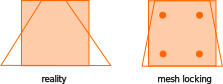
\includegraphics[width=0.8\textwidth]{figs/mesh-locking.png}
 \end{figure}
\end{frame}

\note{
	The neutral axis is the line $y = 0$, and cross-sections, which are initially perpendicular to the neutral axis, are deìned by lines of constant $x$. If the element is subjected to applied moments on the left and right edges, the resulting deformation is bilinear. As shown, it is symmetric about $x = 0$:
	
	\begin{align*}
		u & = \delta \frac{x}{b}\frac{y}{h} \\
		v & = 0
	\end{align*}
	
	Differentiating, the strain, as a function of $x$ and $y$:
	
	\begin{align*}
		\epsilon_{11} &= \frac{\delta y}{bh} \\
		\epsilon_{2} &= 0 \\
		\epsilon_{11} &= \frac{\delta x}{2bh}
	\end{align*}
}

\note{
	\textbf{Volume Locking}
	The volume strain is $\epsilon_{11} + \epsilon_{22} + \epsilon_{33}$. In plane strain , $\epsilon_{33}$ is always zero. An incompressible material in plane strain therefore requires $\epsilon_{22} = -\epsilon_{11}$. Looking at strain equation, $\epsilon_{22}$ must be linear in $y$ just like $\epsilon_{33}$ to satisfy the incompressibility constraint.
}

\note{
	This demonstrates that a quadrilateral element with linear shape functions can't satisfy the incompressibility constraint exactly in bending. Even if we ignore the impossibility of satisfying the incompressibility constraint pointwise throughout the element, it's also clear that the constraint can't be satisfied at the Gauss points for 2 x 2 integration because the sign of $\epsilon_{22}$ must change sign between the upper and lower rows of integration points. The sign change implies that $\epsilon_{22}$ must be at least linear in $y$, which therefore implies that $v$ must be at least quadratic in $y$. There is one point where the incompressibility constraint is satisfied for the bending mode, namely the element centroid. The incompressibility constraint is, therefore, usually imposed at the element centroid in 4-node quadrilateral and 8-node brick elements.
}
\note{
	Use reduced integration method to ``soften'' the element.
	\begin{itemize}
		\item 4 node isoparametric element uses 4 integration points, but one point in the middle in reduced integration. 
		\item The solution may be affected by the mesh size and mesh instability. Need to investigate there are no problmes before the analysis. 
		\item This problem is because of lower order FEs.
	\end{itemize}

	Use selectively reduced integration method
	\begin{itemize}
		\item Volumetirc and deviatoric strains are decomposed and different integration schemes are used.
		\item Some commercial programs have this capability
	\end{itemize}
}

%------------------------------------------------
\begin{frame}
\frametitle{Modeling considerations: Element geometries}
\mode<beamer>{
	\begin{enumerate}
		\item if $det(\mathbf{J}^e)$ is zero, an area element in the parent element is mapped into a zero area in the physical element, which is not acceptable.
		\item Similarly, if elements are excessively distorted, an area element in the parent element is 	mapped into a nearly zero area.
		
		\item To ensure that $det(\mathbf{J}^e)$ is safely larger than zero, certain severely distorted element shapes must be avoided.
	\end{enumerate}
}
\mode<handout>{
	\vspace{3cm}
}
\begin{figure}[ht]
	\centering
	\includegraphics[width=0.8\textwidth]{figs/illformed-quadrilaterals.png}
	\caption*{Quadrilateral element geometries to be avoided.}
\end{figure}
\end{frame}

%------------------------------------------------
\begin{frame}
\frametitle{Modeling considerations: Higher-order element}
Notice for higher order elements, like the nine-noded one, the position of the mid-nodes
contribute to the element distortion. Therefore, they must lie at a certain distance from
the corner nodes.
\mode<beamer>{
	\begin{figure}[ht]
		\centering
		\includegraphics[width=0.8\textwidth]{figs/acceptable-nodal-locations-quadrilateral.png}
		\caption*{Range of acceptable positions for the midnodes of a nine-node quadrilateral element.}
	\end{figure}
}
\mode<handout>{
	\vspace{3cm}
}

\end{frame}
\end{document}